% allgem. Dokumentenformat
\documentclass[a4paper,12pt,headsepline]{scrartcl}
%Variablen welche innerhalb der gesamten Arbeit zur Verfügung stehen sollen
\newcommand{\titleDocument}{Nichtlineare Dynamik und Kontrolle SS 2015}
\newcommand{\subjectDocument}{Projekt 2: Synchronisation in Netzwerken: Master Stability Function und
	Permutationssymmetrien}

% weitere Pakete
% Grafiken aus PNG Dateien einbinden
\usepackage{graphicx}

% Deutsche Sonderzeichen benutzen 
\usepackage{ngerman}

% deutsche Silbentrennung
\usepackage[ngerman]{babel}

% Eurozeichen einbinden
\usepackage[right]{eurosym}

% Umlaute unter UTF8 nutzen
\usepackage[utf8]{inputenc}

% Zeichenencoding
\usepackage[T1]{fontenc}

\usepackage{lmodern}
\usepackage{fix-cm}

% floatende Bilder ermöglichen
%\usepackage{floatflt}

% mehrseitige Tabellen ermöglichen
\usepackage{longtable}

% Unterstützung für Schriftarten
%\newcommand{\changefont}[3]{ 
%\fontfamily{#1} \fontseries{#2} \fontshape{#3} \selectfont}

% Packet für Seitenrandabständex und Einstellung für Seitenränder
\usepackage{geometry}
\geometry{left=3.5cm, right=2cm, top=2.5cm, bottom=2cm}

% Paket für Boxen im Text
\usepackage{fancybox}

% bricht lange URLs "schoen" um
\usepackage[hyphens,obeyspaces,spaces]{url}

% Paket für Textfarben
\usepackage{color}

% Mathematische Symbole importieren
\usepackage{amssymb}
\usepackage{amsmath}

% auf jeder Seite eine Überschrift (alt, zentriert)
%\pagestyle{headings}

% erzeugt Inhaltsverzeichnis mit Querverweisen zu den Kapiteln (PDF Version)
\usepackage[bookmarksnumbered,pdftitle={\titleDocument},hyperfootnotes=false]{hyperref} 
%\hypersetup{colorlinks, citecolor=red, linkcolor=blue, urlcolor=black}
%\hypersetup{colorlinks, citecolor=black, linkcolor= black, urlcolor=black}

% neue Kopfzeilen mit fancypaket
\usepackage{fancyhdr} %Paket laden
\pagestyle{fancy} %eigener Seitenstil
\fancyhf{} %alle Kopf- und Fußzeilenfelder bereinigen
\fancyhead[L]{\nouppercase{\leftmark}} %Kopfzeile links
\fancyhead[C]{} %zentrierte Kopfzeile
\fancyhead[R]{\thepage} %Kopfzeile rechts
\renewcommand{\headrulewidth}{0.4pt} %obere Trennlinie
%\fancyfoot[C]{\thepage} %Seitennummer
%\renewcommand{\footrulewidth}{0.4pt} %untere Trennlinie

% für Tabellen
\usepackage{array}

% Runde Klammern für Zitate
%\usepackage[numbers,round]{natbib}

% Festlegung Art der Zitierung - Havardmethode: Abkuerzung Autor + Jahr
\bibliographystyle{alphadin}

% Schaltet den zusätzlichen Zwischenraum ab, den LaTeX normalerweise nach einem Satzzeichen einfügt.
\frenchspacing

% Paket für Zeilenabstand
\usepackage{setspace}

% für Bildbezeichner
\usepackage{capt-of}

% für Stichwortverzeichnis
\usepackage{makeidx}


% Indexerstellung
\makeindex
\numberwithin{equation}{subsection}

% Disable single lines at the start of a paragraph (Schusterjungen)
\clubpenalty = 10000
% Disable single lines at the end of a paragraph (Hurenkinder)
\widowpenalty = 10000
\displaywidowpenalty = 10000

\begin{document}
% hier werden die Trennvorschläge inkludiert
%hier müssen alle Wörter rein, welche Latex von sich auch nicht korrekt trennt bzw. bei denen man die genaue Trennung vorgeben möchte
\hyphenation{
Film-pro-du-zen-ten
Lux-em-burg
Soft-ware-bau-steins
zeit-in-ten-siv
}

%Schriftart Helvetica
%\changefont{phv}{m}{n}

% Leere Seite am Anfang


% Titelseite %
% das Papierformat zuerst
%\documentclass[a4paper, 11pt]{article}

% deutsche Silbentrennung
%\usepackage[ngerman]{babel}

% wegen deutschen Umlauten
%\usepackage[ansinew]{inputenc}

% hier beginnt das Dokument
%\begin{document}


\thispagestyle{empty}

\begin{figure}[t]

 
\includegraphics[width=0.3\textwidth]{abb/misc/TULogo.eps}
~~~~~~~~~~
\end{figure}


\begin{verbatim}


\end{verbatim}

\begin{center}
\Large{Technische Universit\"at Berlin}\\
\end{center}


\begin{center}
\Large{Fakult\"at II Mathematik und Naturwissenschaften}
\end{center}
\begin{verbatim}


\end{verbatim}
\begin{center}
\doublespacing
\textbf{\LARGE{\titleDocument}}\\
\singlespacing
\begin{verbatim}

\end{verbatim}
\textbf{{~\subjectDocument}}
\end{center}
\begin{verbatim}

\end{verbatim}
\begin{center}

\end{center}
\begin{verbatim}





\end{verbatim}
\begin{flushleft}
\begin{tabular}{llll}
\textbf{Autoren:} &  Halgurd Taher &\\& Felix Zimmermann& \\
&  Paul-Rainer Affeld & \\
& & \\
\textbf{Version vom:}  & \today &
\end{tabular}
\end{flushleft}

% römische Numerierung
%\pagenumbering{arabic}

% 1.5 facher Zeilenabstand
\onehalfspacing


% Einleitung / Abstract
\section*{Zusammenfassung}


%\begin{verbatim}

%

%\end{verbatim}

\section*{Abstract}


% einfacher Zeilenabstand
\singlespacing

% Inhaltsverzeichnis anzeigen
\newpage
\thispagestyle{empty}
\tableofcontents


\addcontentsline{toc}{section}{Abbildungsverzeichnis}
\listoffigures


\addcontentsline{toc}{section}{Tabellenverzeichnis}
\listoftables


% Definiert Stegbreite bei zweispaltigem Layout
\setlength{\columnsep}{25pt}

%%%%%%% EINLEITUNG %%%%%%%%%%%%
%\twocolumn
\newpage
\fancyhead[L]{\nouppercase{\leftmark}} %Kopfzeile links

% 1,5 facher Zeilenabstand
\onehalfspacing

% einzelne Kapitel
\section{Einleitung}\label{einleitung}
Dynamische Netzwerke spielen in heutigen Wissenschaft eine wichtige Rolle. So lassen sich beispielsweise Prozesse im Gehirn zwischen Neuronen über Netzwerke beschreiben und analysieren. Großflächige Stromnetze stellen ebenfalls ein klassisches Beispiel eines Netzwerkes dar. Es ist von großem Interesse Prozesse in solchen Systemen hinsichtlich Dynamik und Stabilität zu untersuchen. Ein bekanntes Hilfmittel zur Analyse von Netzwerken ist die sogenannte Master Stability Function (MSF), mit deren Hilfe sich Aussagen über die Stabilität von globalen Synchronisationszuständen treffen lassen.\\
Bei der Betrachtung der real existierenden Netzwerke können allerdings (häufiger als globale Synchronisation) Cluster aus synchronen Knoten (Nervenzellen, Kraftwerke) beobachtet werden. So spielt bei verscheidenen Erkrankungen wie fokaler Epilepsie das Auftreten synchroner Areale im Gehirn eine entscheidende Rolle zur Pathogenese.\\
Ziel dieser Ausarbeitung ist es, eine Methode zu präsentieren und zu verifizieren mit der nicht nur eine globale Analyse des Netzwerkes möglich ist, sondern auch die Clusterbildung und lokales Verhalten dieser Cluster untersucht werden kann.


\section{Netzwerke}
Netzwerke setzen sich im allgmeinen aus $N$ Knoten (Nodes) zusammen, die über gewichtete Verbindungen (Edges) miteinander verbunden sind. Besteht zwischen zwei Knoten eine Verbindung in beide Richtungen, so spricht man von einem ungerichteten Netzwerk. Wenn alle Knoten untereinander verbunden sind, so handelt es sich um ein vollständiges Netzwerk (siehe Abbildung \ref{fig:GraphBsp}). Die Verbindungen der Knoten lassen sich durch eine $M\times M$ Verbindungsmatrix $\boldsymbol{A}$ darstellen, in der ein Eintrag von $1$ an Position $i,j$ eine Verbindung zwischen dem Knoten $i$ und dem Knoten $j$, eine $0$ keine Verbindung zwischen diesen Knoten bedeutet.

\begin{figure}[t]
	 \centering
	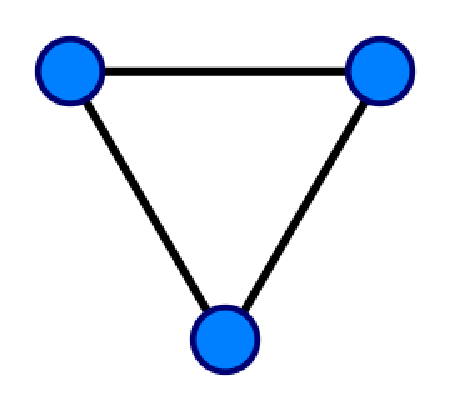
\includegraphics[width=0.25\textwidth]{abb/misc/GraphBsp.eps}
	\caption[Ungerichteres Netzwerk]{Beispiel eines ungerichteten Netzwerks aus vier Knoten, bei dem jeder Knoten mit jedem anderen verbunden ist.}
	\label{fig:GraphBsp}
\end{figure}


\subsection*{Dynamik auf Netzwerken}
Um Prozesse auf Netzwerken zu beschreiben kann man jedem Knoten eine $n$-dimensionale dynamische Variable $x_i$ zuordnen. Die Dynamik wird dann für jeden Knoten über eine Differentialgleichung beschrieben, die die Kopplung an die anderen Knoten enthält. Die allgemeine Form dieser Differentialgleichung ist in Gleichung (\ref*{eq:dyneqcommon}) gezeigt.

%was ist das mit der rückkopplung? die ist doch da drin? haben wir mal rausgenommen

\begin{align}\label{eq:dyneqcommon}
\overset{\cdot}{\boldsymbol{x}}_i(t)&=\boldsymbol{f}(\boldsymbol{x}_i(t))+\sigma\sum_j A_{ij}\boldsymbol{h}\left(\boldsymbol{x}_j(t)\right)
\\\notag & i=1,...,N
\\\notag & \sigma \text{ allgemeine Kopplungsstärke}
\\\notag & A_{ij}\text{ Element der Kopplungsmatrix}
\\\notag & \boldsymbol{f},\boldsymbol{h}:\mathbb{R}^n\rightarrow\mathbb{R}^n
\end{align}
Die Verbindungsmatrix $\boldsymbol{A}$ wird hierbei zu einer Kopplungsmatrix, die die Kopplung der Differentialgleichungen der Knoten untereinander beschreibt. Im folgenden werden nur solche Systeme betrachtete, bei denen $\boldsymbol{A}$ symmetrisch ist, das Netzwerk also ungerichtet. Die Abbildung $\boldsymbol{h}$ beschreibt auf welche Art und Weise die Komponenten der Variablen $\boldsymbol{x}_i$ aneinander koppeln. Das Differentialgleichungssystem in (\ref*{eq:dyneqcommon}) lässt sich auch über das Kronecker-Produkt in einer einzigen Gleichung darstellen \citep{pecora1998},
\begin{align}
\overset{\cdot}{\boldsymbol{X}}(t)=\boldsymbol{F}(\boldsymbol{X}(t))+\sigma\boldsymbol{A}\otimes\boldsymbol{H}(\boldsymbol{X}(t))
\end{align}
mit den Definitionen:
\begin{align*}
\boldsymbol{X}=\left(\boldsymbol{x}_1,...,\boldsymbol{x}_N\right)^{\text{T}},
\boldsymbol{F}=\left(\boldsymbol{f}(\boldsymbol{x}_1),...,\boldsymbol{f}(\boldsymbol{x}_N)\right)^{\text{T}},
\boldsymbol{H}=\left(\boldsymbol{h}(\boldsymbol{x}_1),...,\boldsymbol{h}(\boldsymbol{x}_N)\right)^{\text{T}}
\end{align*}



\section{Synchronisation}
\subsection*{Globale Synchronisation}
Das Netzwerk wird als global synchron bezeichnet, wenn sich alle Variablen $\boldsymbol{x}_i$ zeitlich gleich verhalten.
\begin{align*}
\boldsymbol{x}_1(t)=\boldsymbol{x}_2(t)=...=\boldsymbol{x}_N(t)=:\boldsymbol{s}(t)
\end{align*}
Es spielt dabei keine Rolle, ob dieses Verhalten z.B konstant, periodisch oder chaotisch ist.

\subsection*{Isolierte Synchronisation}
Isolierte Synchronisation liegt vor, wenn eine Gruppe von Knoten oben genanntes Verhalten aufweist, während ein anderer Teil des Netzwerks nicht synchron mit dieser Gruppe ist.



%....

\section{Ausblick}\label{ausblick}

\section{Fazit}\label{fazit}

%% Beispiel für Bild mit Fußnote
\begin{figure}[htb]
 \centering
 \includegraphics[width=0.4\textwidth,angle=45]{abb/logo1}
 \caption[Beispiel einer Bildbeschreibung]{Beispiel einer Bildbeschreibung\footnotemark}
\label{fig:beispiel1}
\end{figure}
\footnotetext{Bildquelle: Beispielquelle}

% Beispiel für Bildintegration
\begin{figure}[htb]
 \centering
 \includegraphics[width=0.3\textwidth,angle=0]{abb/logo2}
 \caption[Beschreibung]{Beschreibung}
\label{fig:Beschreibung}
\end{figure}

% Beispiel: Referenz auf Abbildung
Abbildung~\ref{fig:Beschreibung} [S.\pageref{fig:Beschreibung}]

% Beispiel: Tabelle 
\begin{center}
  \begin{tabular}{ | l | c | }
    \hline
    Überschrift 1 & Überschrift 2 \\ \hline \hline
    Info 1 & Info 2 \\ \hline
    Info 3 & Info 4 \\
    \hline
  \end{tabular}
\end{center}


% Beispiel für Quellcode Listings
\lstset{language=xml}
\begin{lstlisting}[frame=htrbl, caption={Die Datei {\tt data-config.xml} dient als Beispiel für XML Quellcode}, label={lst:dataconfigxml}]
<dataConfig>
  <dataSource type="JdbcDataSource" 
              driver="com.mysql.jdbc.Driver"
              url="jdbc:mysql://localhost/bms_db"
              user="root" 
              password=""/>
  <document>
    <entity name="id"
        query="select id, htmlBody, sentDate, sentFrom, subject, textBody
        from mail">
    <field column="id" name="id"/>
    <field column="htmlBody" name="text"/>
    <field column="sentDate" name="sentDate"/>
    <field column="sentFrom" name="sentFrom"/>
    <field column="subject"  name="subject"/>
    <field column="textBody" name="text"/>
    </entity>
  </document>
</dataConfig>
\end{lstlisting}

\lstset{language=java}
\begin{lstlisting}[frame=htrbl, caption={Das Listing zeigt Java Quellcode}, label={lst:result2}]
/* generate TagCloud */
Cloud cloud = new Cloud();
cloud.setMaxWeight(_maxSizeOfText);
cloud.setMinWeight(_minSizeOfText);
cloud.setTagCase(Case.LOWER);
	    
/* evaluate context and find additional stopwords */
String query = getContextQuery(_context);
List<String> contextStoplist = new ArrayList<String>();
contextStoplist = getStopwordsFromDB(query);
	    
/* append context stoplist */
while(contextStoplist != null && !contextStoplist.isEmpty())
  _stoplist.add(contextStoplist.remove(0));
	    
/* add cloud filters */
if (_stoplist != null) {
  DictionaryFilter df = new DictionaryFilter(_stoplist);
  cloud.addInputFilter(df);
}
/* remove empty tags */
NonNullFilter<Tag> nnf = new NonNullFilter<Tag>();
cloud.addInputFilter(nnf);

/* set minimum tag length */
MinLengthFilter mlf = new MinLengthFilter(_minTagLength);
cloud.addInputFilter(mlf);

/* add taglist to tagcloud */
cloud.addText(_taglist);

/* set number of shown tags */	    
cloud.setMaxTagsToDisplay(_tagsToDisplay);
\end{lstlisting}


% Beispiel für Formeln
Die Zuordnung aller möglichen Werte, welche eine Zufallsvariable annehmen kann nennt man \emph{Verteilungsfunktion} von $X$.

\begin{quotation}
Die Funktion F: $\mathbb{R} \rightarrow$ [0,1] mit $F(t) = P (X \le t)$ heißt Verteilungsfunktion von $X$.\footnote{Konen, vgl.~\cite{wk05}~[S.55]}
\end{quotation}

\begin{quotation}
Für eine stetige Zufallsvariable $X: \Omega \rightarrow \mathbb{R}$ heißt eine integrierbare, nichtnegative reelle Funktion $w: \mathbb{R} \rightarrow \mathbb{R}$ mit $F(x) = P(X \le x) = \int_{-\infty}^{x} w(t)dt$ die \emph{Dichte} oder \emph{Wahrscheinlichkeitsdichte} der Zufallsvariablen $X$.\footnote{Konen, vgl.~\cite{wk05}~[S.56]}
\end{quotation}


\onecolumn
% einfacher Zeilenabstand
\singlespacing
% Literaturliste soll im Inhaltsverzeichnis auftauchen
\newpage
\addcontentsline{toc}{section}{Literaturverzeichnis}
% Literaturverzeichnis anzeigen
\renewcommand\refname{Literaturverzeichnis}
\bibliography{Hauptdatei}

%% Index soll Stichwortverzeichnis heissen
% \newpage
% % Stichwortverzeichnis soll im Inhaltsverzeichnis auftauchen
% \addcontentsline{toc}{section}{Stichwortverzeichnis}
% \renewcommand{\indexname}{Stichwortverzeichnis}
% % Stichwortverzeichnis endgueltig anzeigen
% \printindex

\onehalfspacing
% evtl. Anhang
\newpage
\addcontentsline{toc}{section}{Anhang}
\fancyhead[L]{Anhang} %Kopfzeile links
\subsection*{Anhang}\label{anhang}



% leere Abschlussseite
%\newpage
%\thispagestyle{empty} % erzeugt Seite ohne Kopf- / Fusszeile
%\section*{ }

\end{document}